% build/cover.tex — 表紙を単独で生成するLaTeXファイル
\documentclass[a4paper]{article}
\usepackage[margin=0pt]{geometry}
\usepackage{tikz}
\usepackage{graphicx}
\usepackage{fontspec}
\usepackage[haranoaji]{luatexja-preset}
\usepackage{eso-pic}

% 表紙用フォント
\newfontfamily\covertitlefont{Noto Serif CJK JP SemiBold}
\newfontfamily\coversubtitlefont{Noto Sans CJK JP}
\newfontfamily\coverauthorfont{Noto Serif CJK JP}

\pagestyle{empty}

\begin{document}
% 背景画像（eso-picで全面配置 — tikzに依存しない）
\AddToShipoutPictureBG*{%
  \AtPageLowerLeft{%
    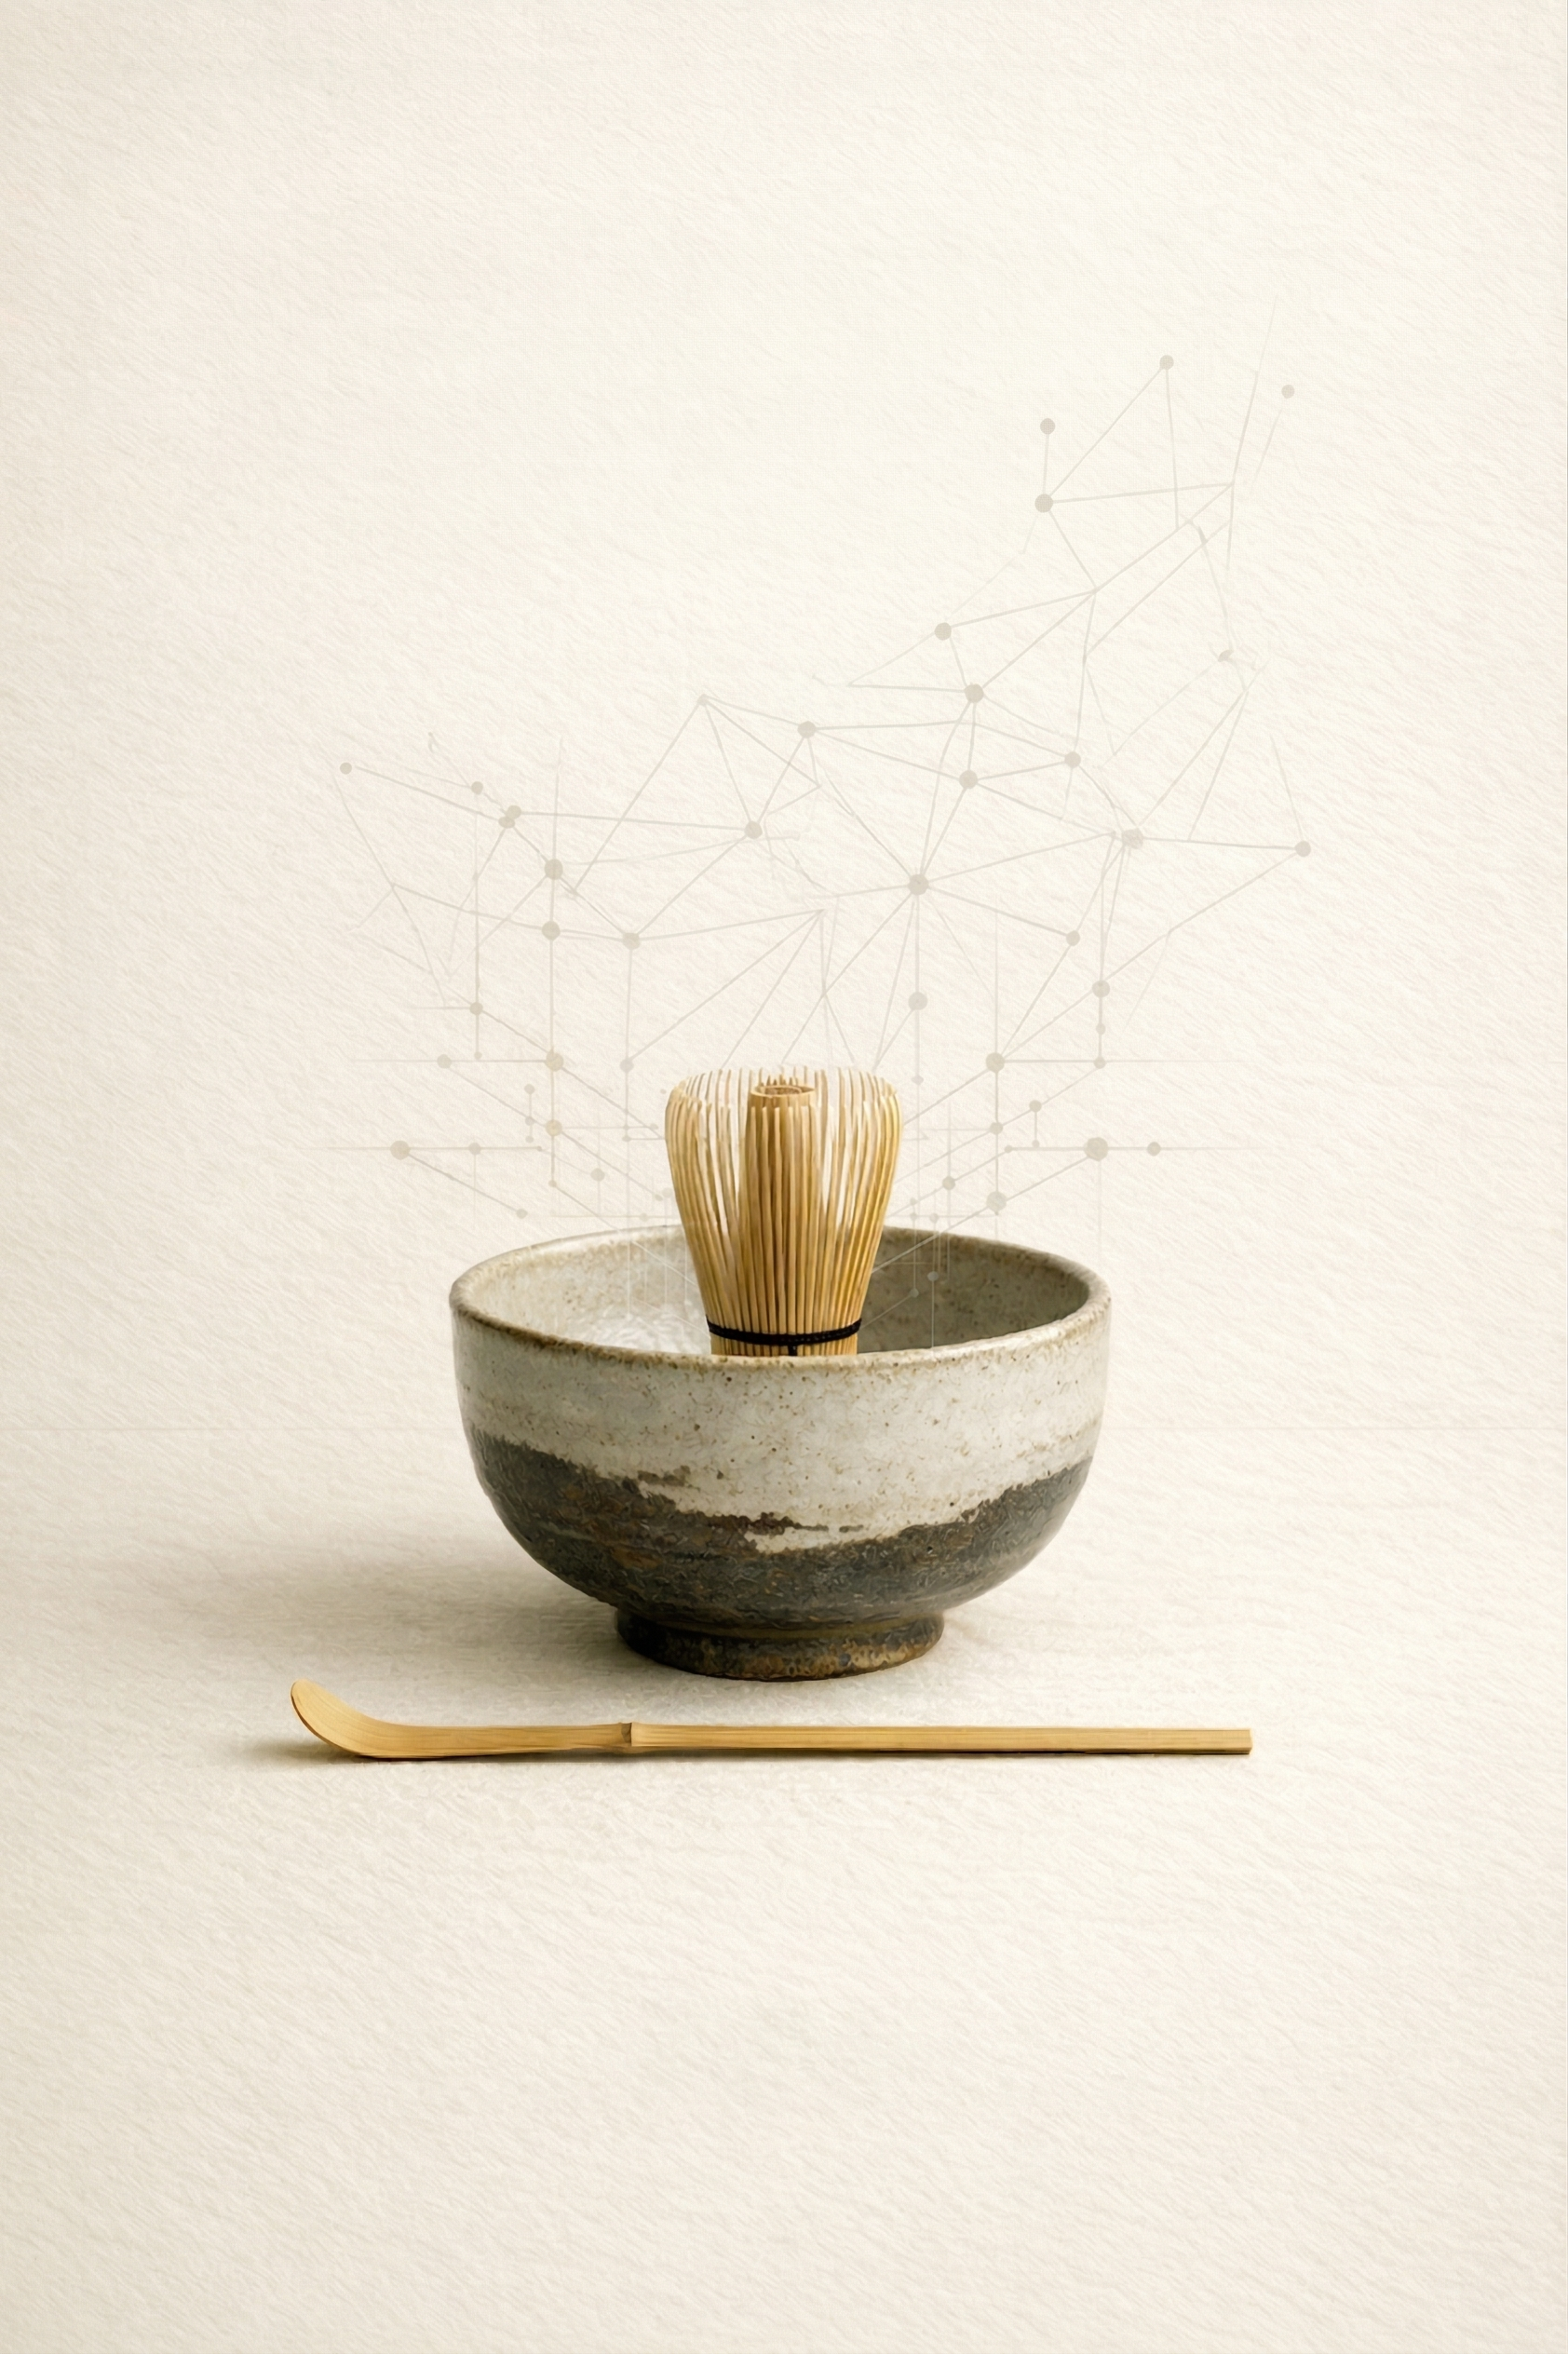
\includegraphics[width=\paperwidth,height=\paperheight]{../figures/cover.jpeg}%
  }%
}

% テキストをtikz overlayで配置
\begin{tikzpicture}[remember picture,overlay]
  % タイトル1行目
  \node[text width=0.78\paperwidth, align=center] at
    ([yshift=-0.14\paperheight]current page.north) {%
      \color[HTML]{1E1E1E}{\fontsize{36}{40}\selectfont\covertitlefont AIエージェントを使いこなす}%
    };
  % タイトル2行目
  \node[text width=0.85\paperwidth, align=center] at
    ([yshift=-0.20\paperheight]current page.north) {%
      \color[HTML]{1E1E1E}{\fontsize{22}{28}\selectfont\covertitlefont はじめてのバイオインフォマティクス開発作法}%
    };
  % 副題
  \node[text width=0.85\paperwidth, align=center] at
    ([yshift=-0.26\paperheight]current page.north) {%
      \color[HTML]{3C3C3C}{\fontsize{12.5}{18}\selectfont\coversubtitlefont 情報技術の基礎から環境構築・設計・テスト・公開まで}%
    };
  % 著者
  \node[align=center] at
    ([yshift=0.10\paperheight]current page.south) {%
      \color[HTML]{1E1E1E}{\fontsize{16}{22}\selectfont\coverauthorfont 二階堂愛}%
    };
\end{tikzpicture}
\end{document}
